% !TEX root =  master.tex
\chapter{Ablaufplan}
\begin{figure}[H]
	\centering 
	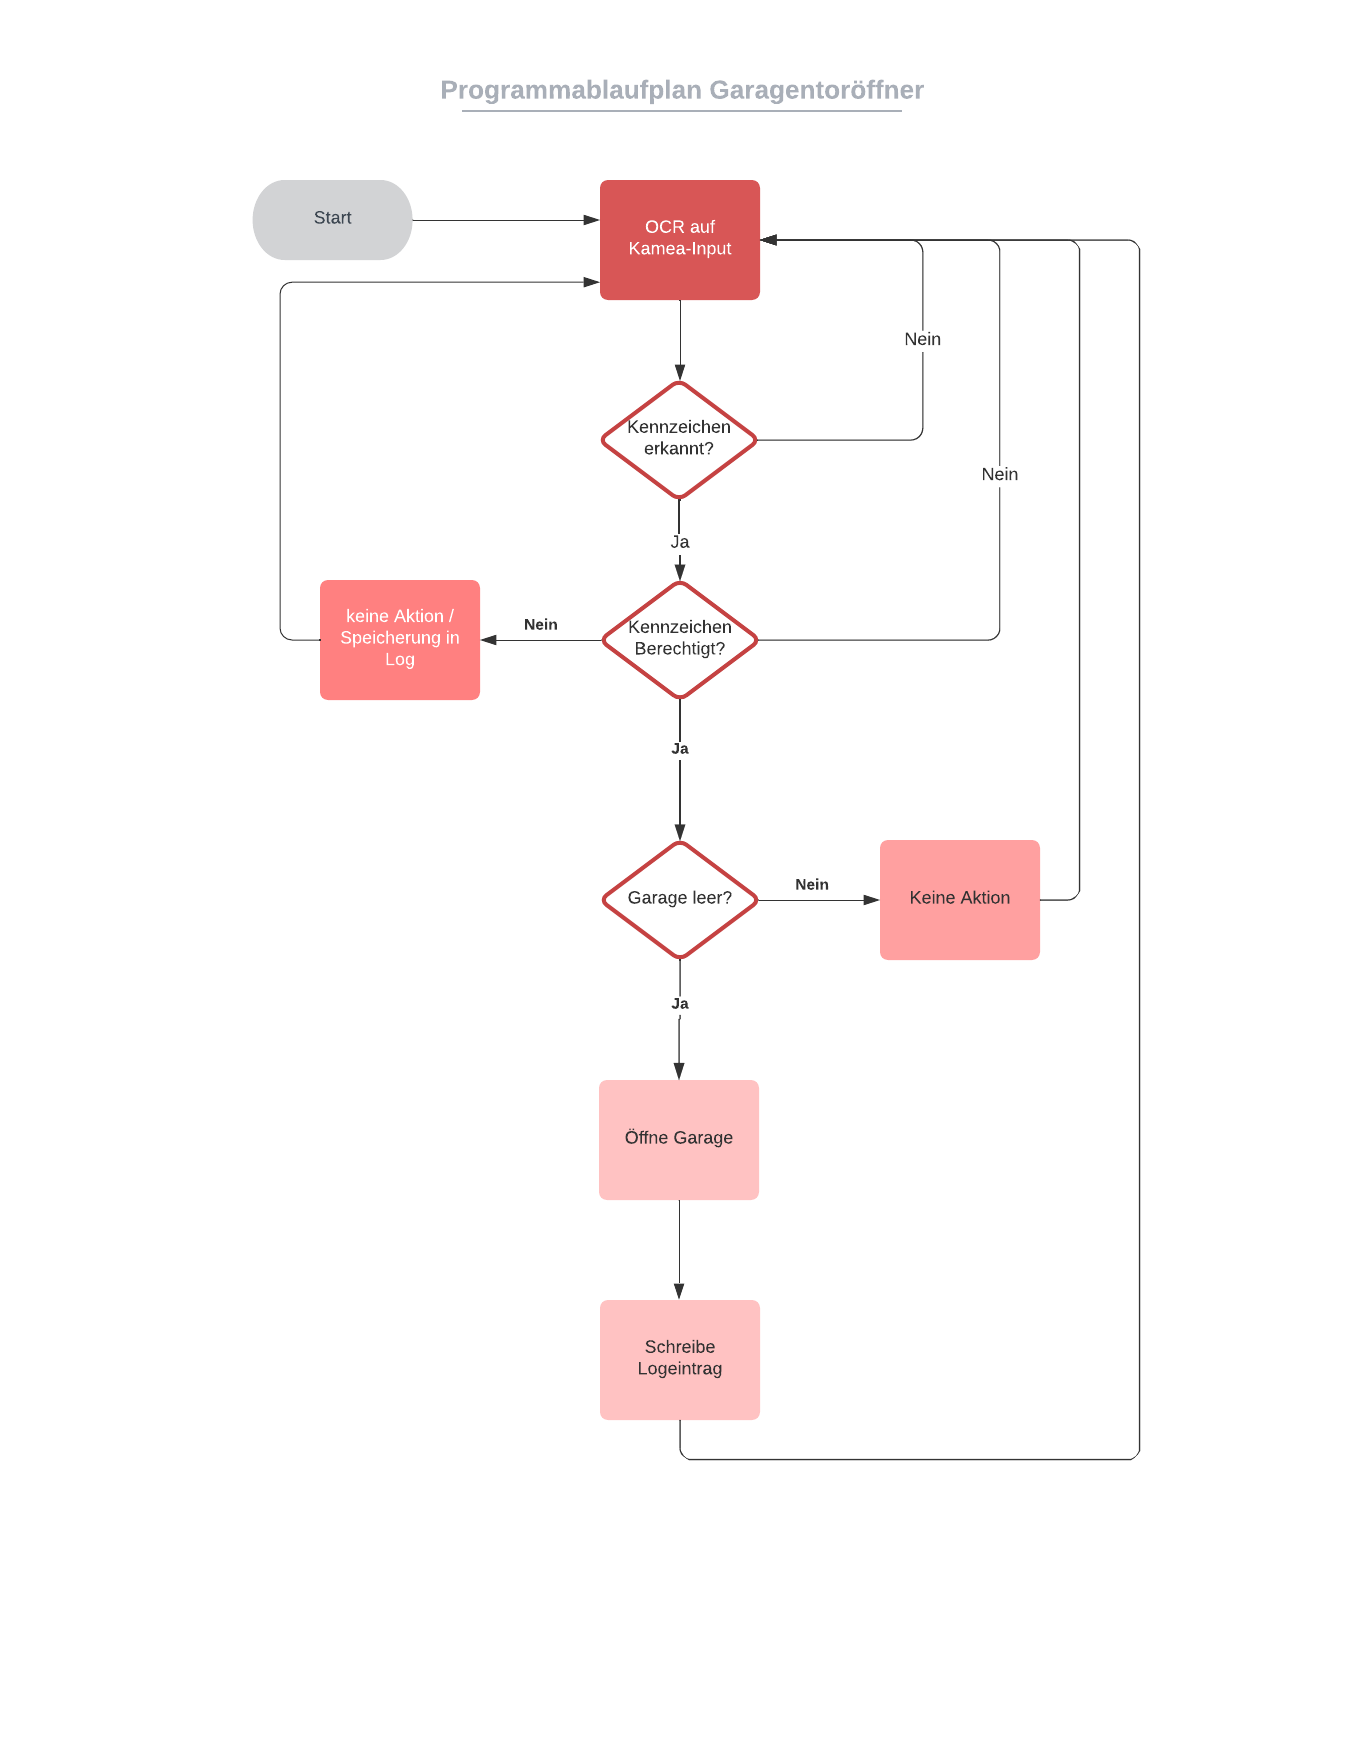
\includegraphics[scale=0.75]{\imagedir/Programmablaufplan.png}
	\captionsetup{format=hang}
	\caption[Programmablauf]{\label{Ablaufplan}Ablauf der Kennzeichenerkennungs-Schleife \\Quelle: Eigene Darstellung}
\end{figure}
\chapter{Schaltplan}
\begin{figure}[h]
	\centering
	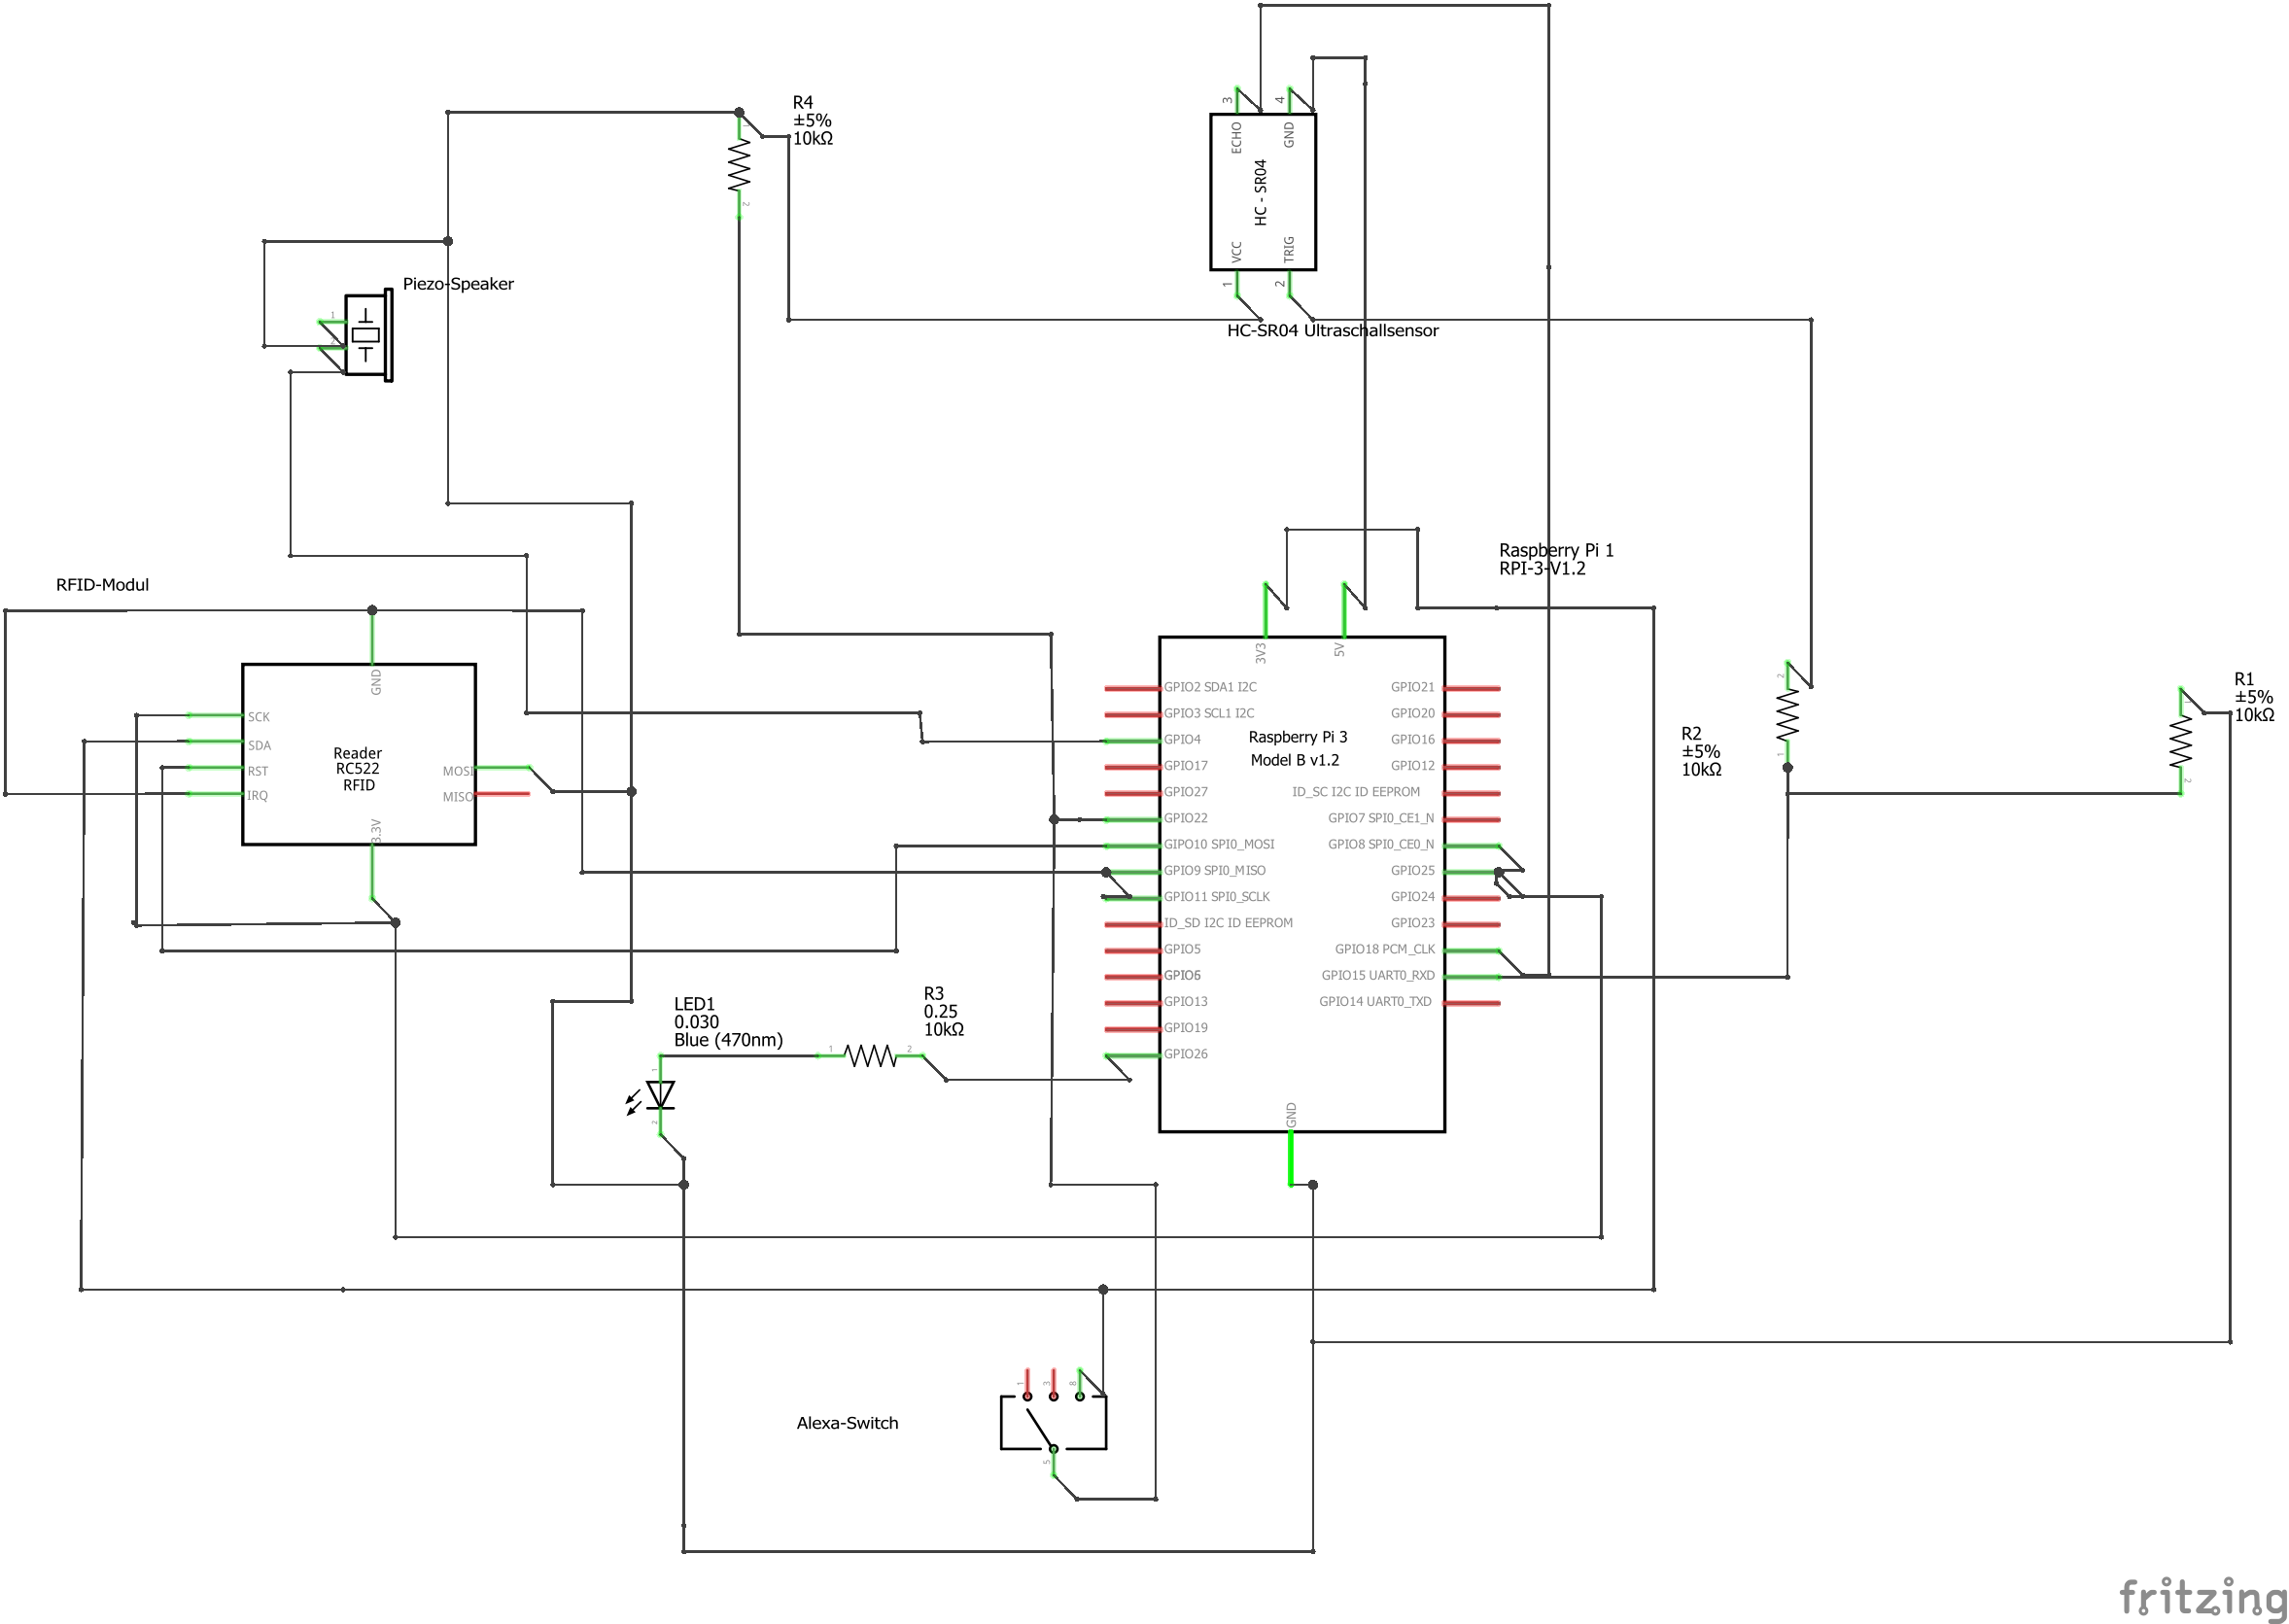
\includegraphics[width=1\linewidth]{img/SmartGarage_Schaltplan}
	\caption{Finaler Schaltplan aller Bauteile \newline Quelle: Eigene Darstellung}
	\label{Schaltplan}
\end{figure}

\chapter{Steckplan}
\begin{figure}[H]
	\centering 
	\label{Steckplan}
	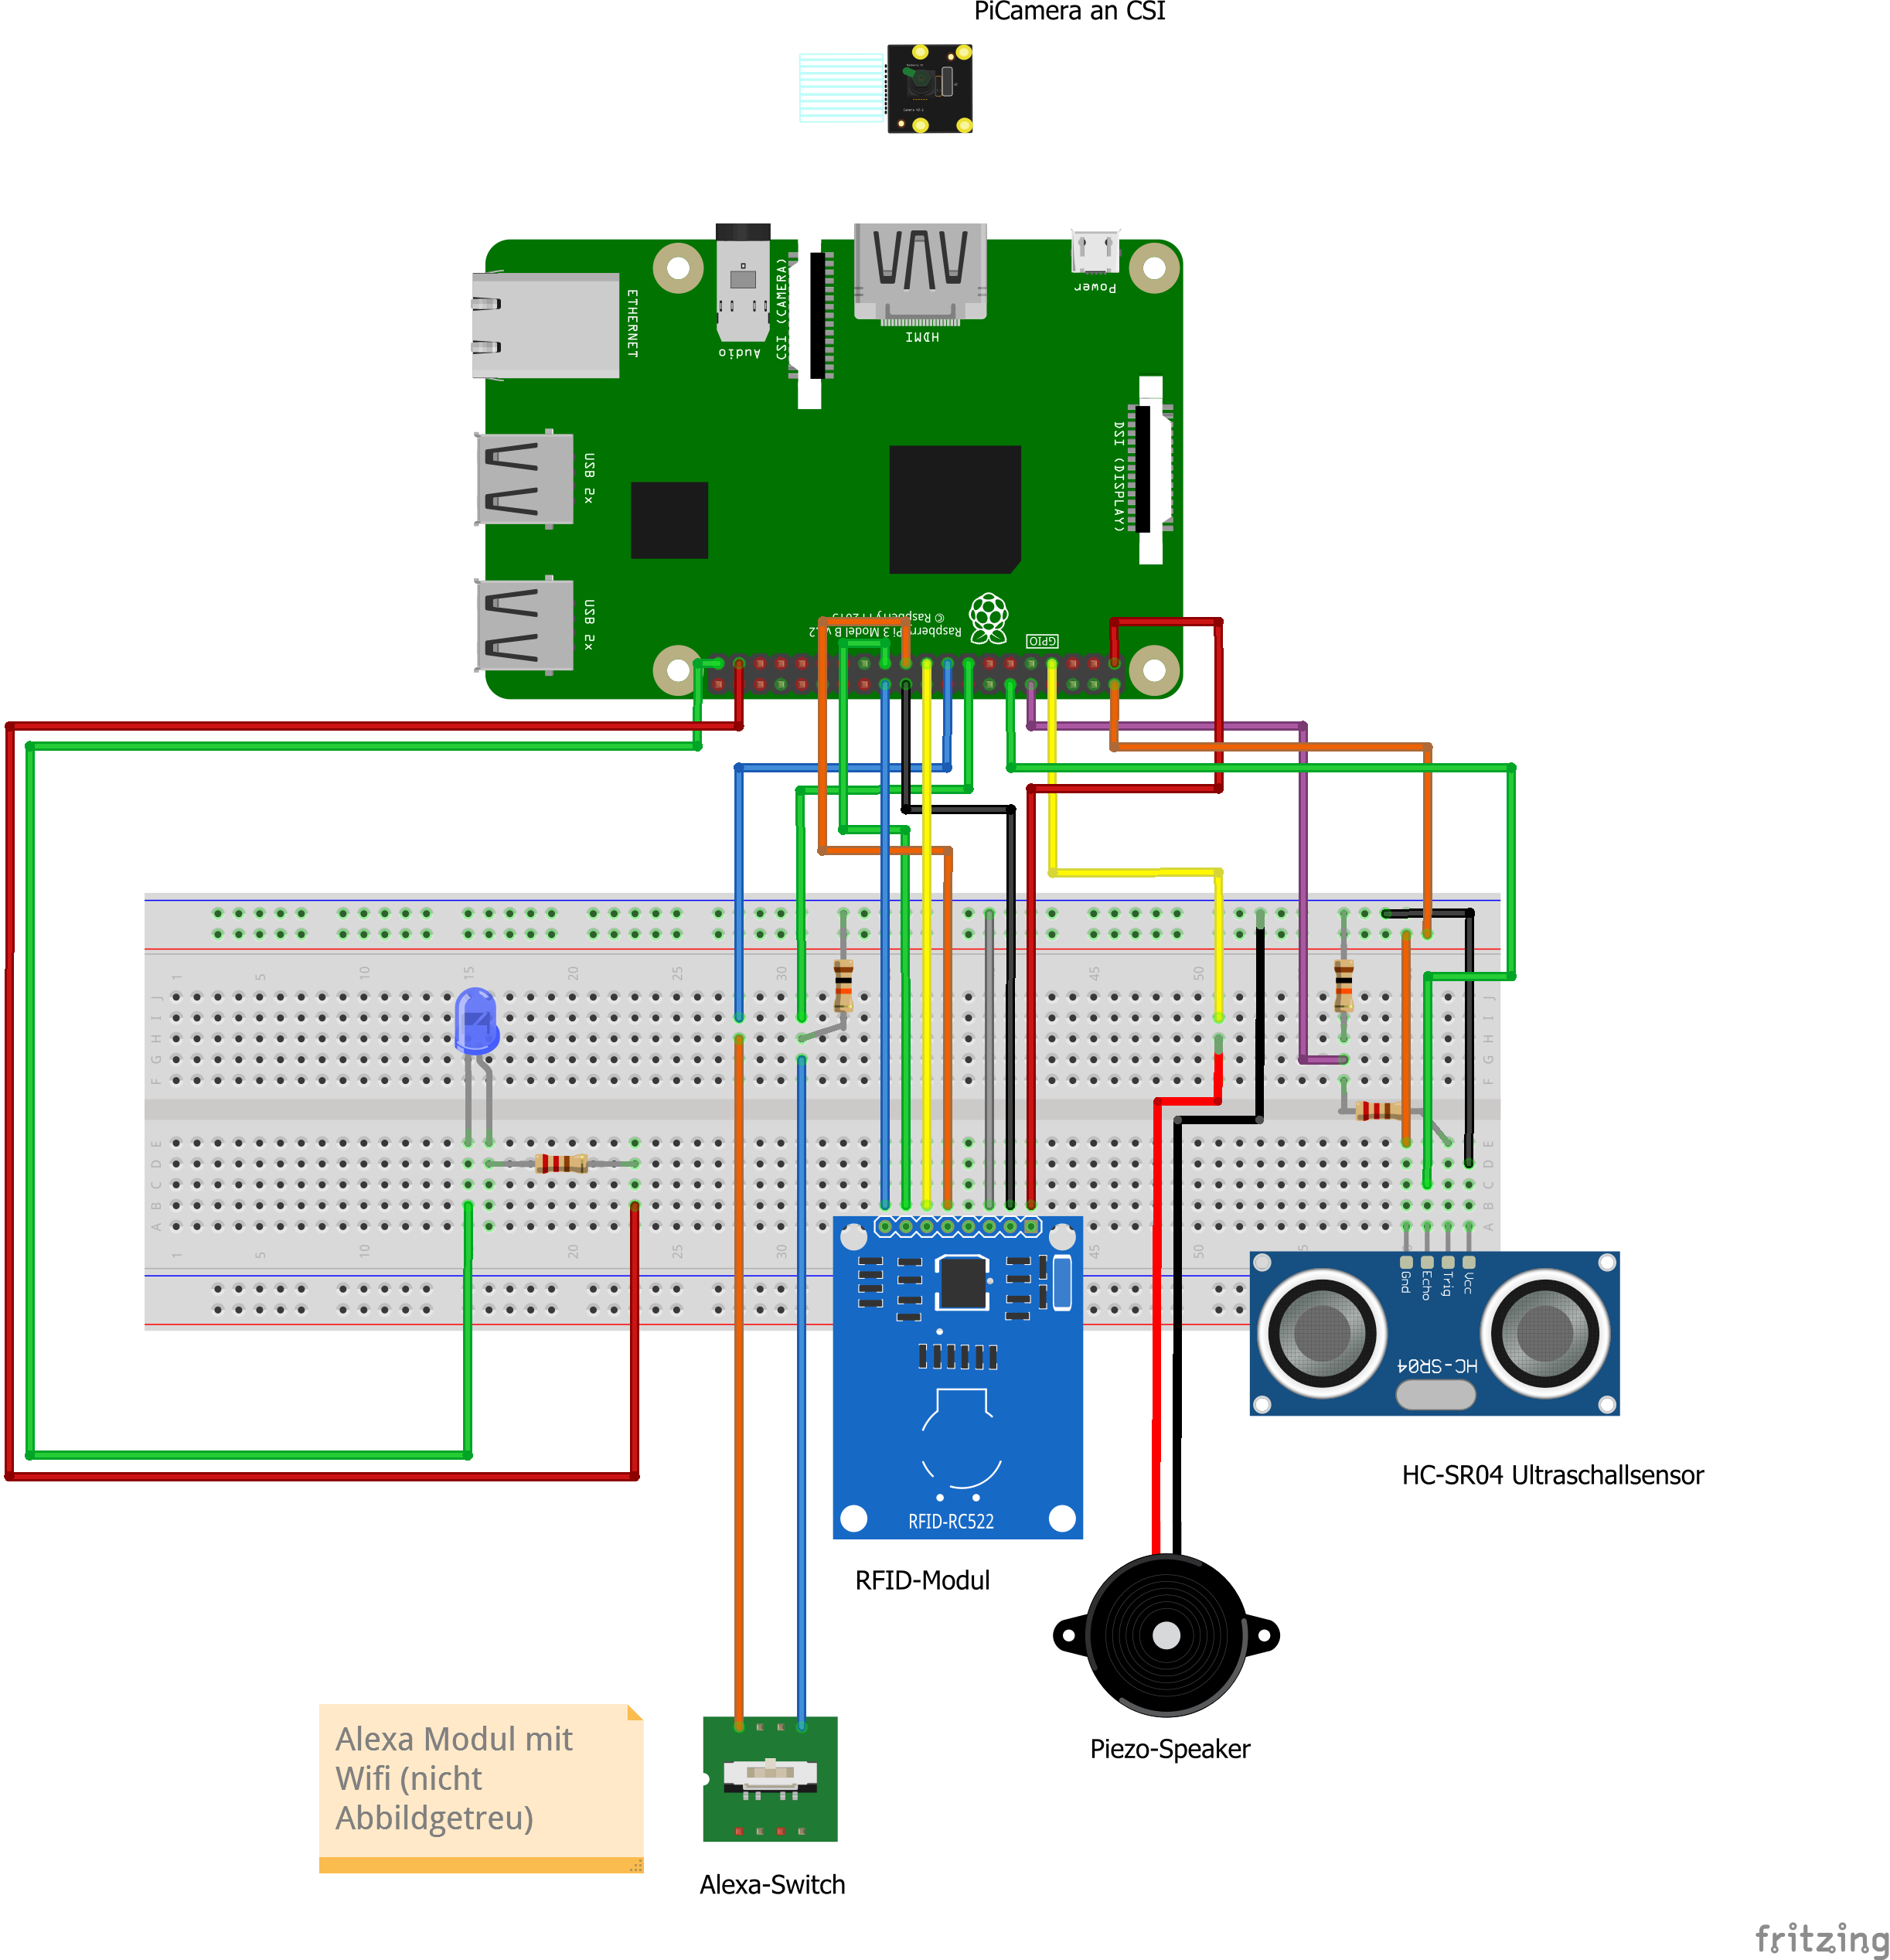
\includegraphics[scale=0.8]{\imagedir/SmartGarage.png}
	\captionsetup{format=hang}
	\caption[Steckplan]{Steckplan der gesamten Hardware \\Quelle: Eigene Darstellung}
\end{figure}
\chapter{Fehlermeldungen}
